% Activate the following line by filling in the right side. If for example the name of the root file is Main.tex, write
% "...root = Main.tex" if the chapter file is in the same directory, and "...root = ../Main.tex" if the chapter is in a subdirectory.
 
%!TEX root =  testMain.tex

\chapter[Simulations to Evaluate Bayesian Networks.]{Creating Simulations to Evaluate Bayesian Networks.}

\section{Introduction}

This chapter lays out the general method for creating simulations with automatic Bayesian Networks, as well as how to evaluate these Bayesian Networks. The general process of creating simulations to evaluate Bayesian Networks is illustrated in Figure~\ref{pipeline}. We start by defining a simulation with agents, and then have reporters report on that simulation in the `Experiment' stage. Relevant events in simulations are collected by the reporters in each run. The collection of runs is used by an automatic Bayesian Network constructor algorithm to construct a Bayesian Network automatically in the `Building BN' stage. Finally, the constructed Bayesian Network is evaluated with respect to the criteria in the `Evaluate BN' stage. These three stages are explained in this section. Specific instances of simulations and networks created with this process are the subject of the next chapters.

\begin{figure}[h]
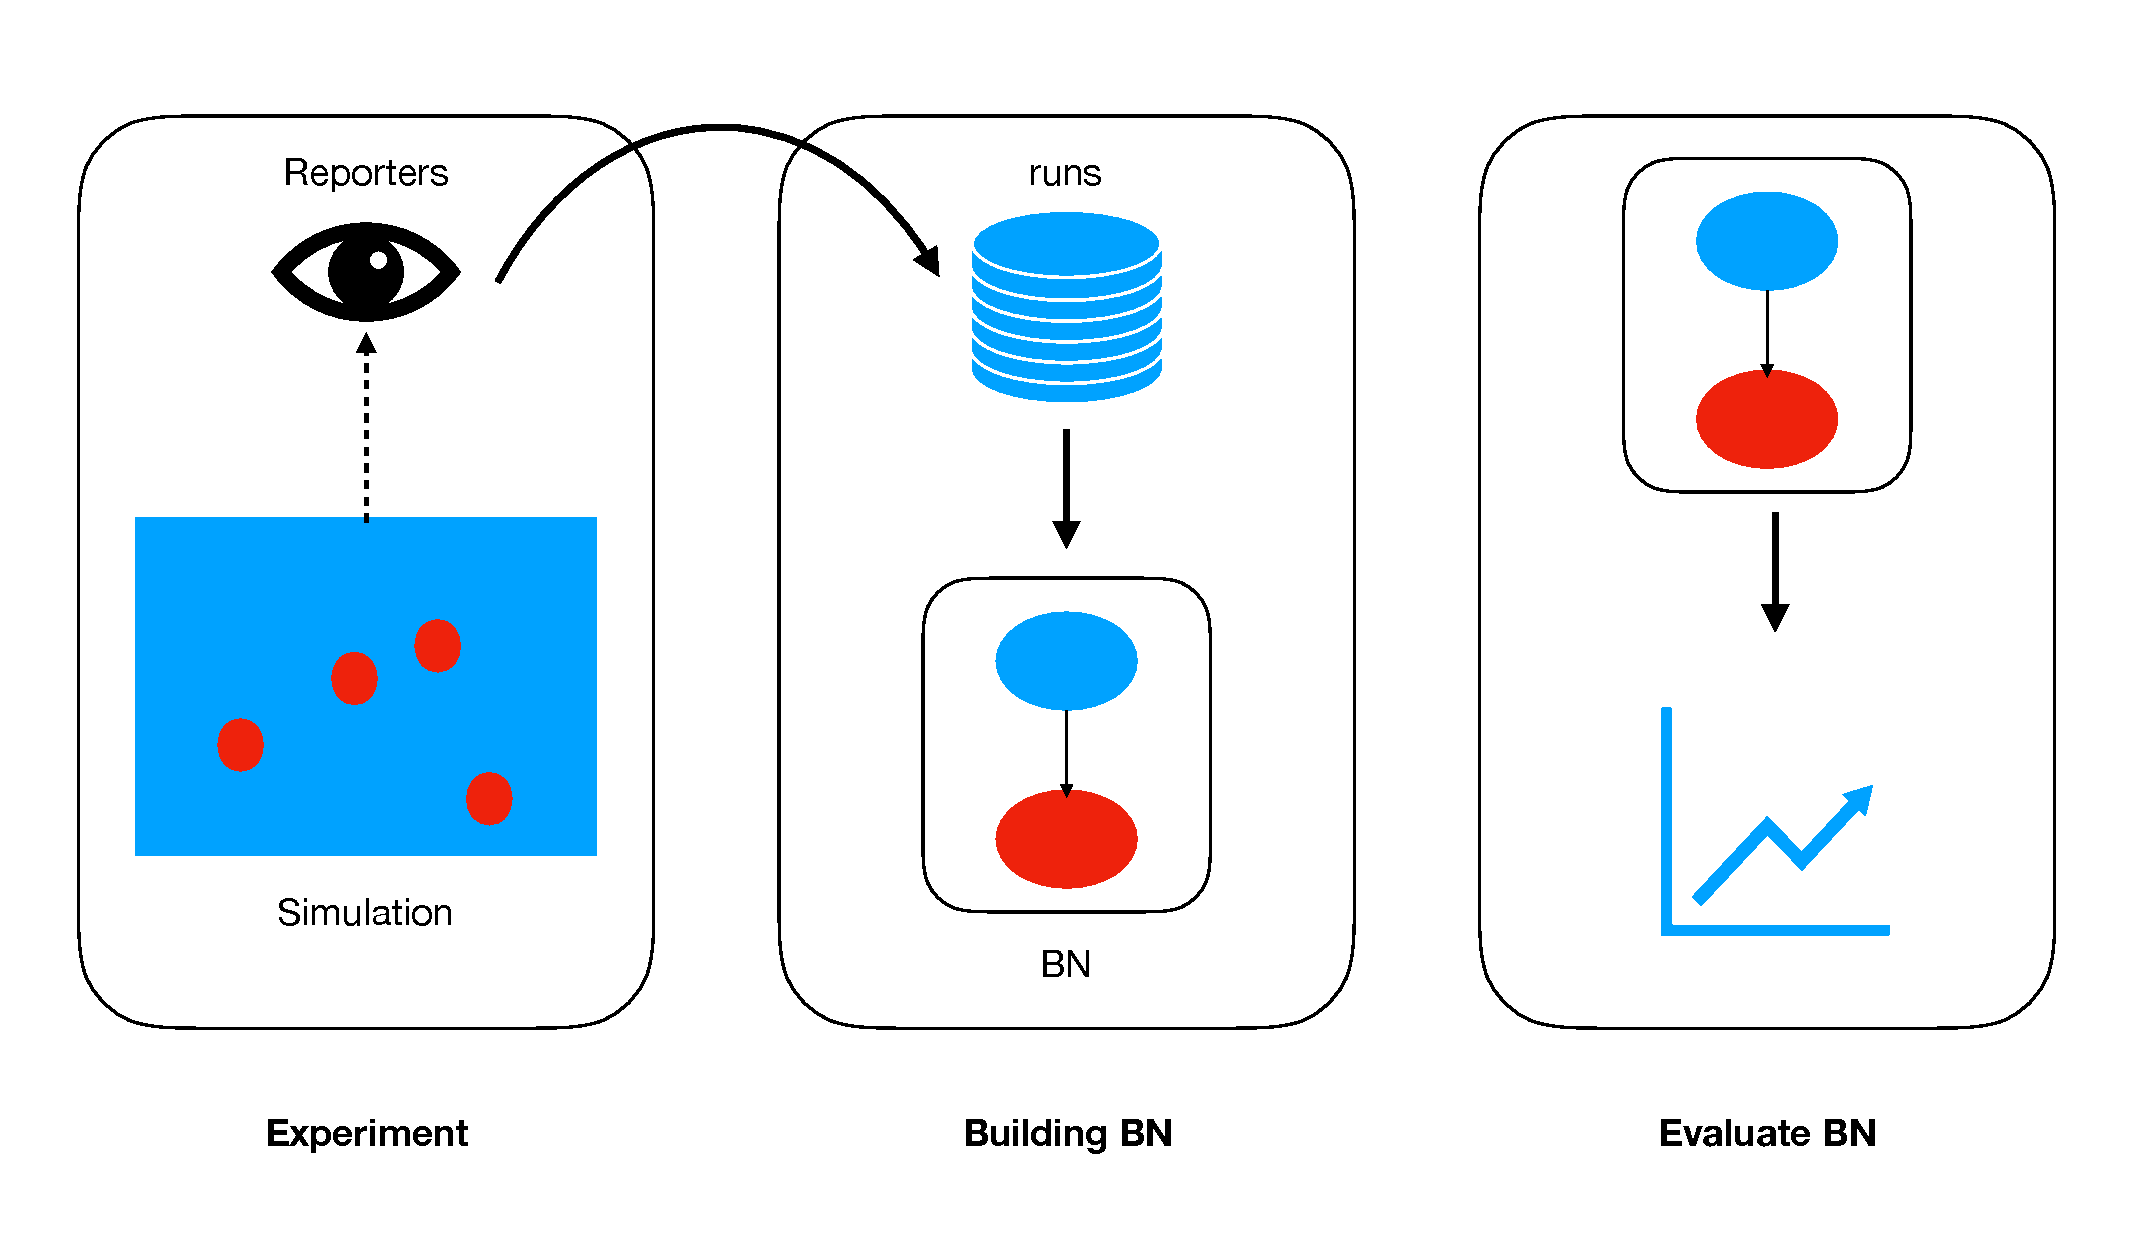
\includegraphics[width=\linewidth]{images/pipeline.pdf}
\caption{Method for evaluating automatically generated Bayesian Networks from simulations.}
\label{pipeline}
\end{figure}


\section{Setting-up an Experiment}
An experiment consists of a simulation and reporters. Reporters are defined separately from the simulation because they are not inherent to it - they are defined with respect to what we want to know about the simulation.

\subsection{Simulation}

\subsubsection{Structure of a simulation}
In the simulation, we are simulating some sort of criminal scenario - a theft, usually. The simulation can be as precise as necessary, but there are certain things that need to be present: we need to have states that can occur and there needs to be evidence for those states. The granularity of the simulation and its complexity depend on the modeller and her requirements.

\subsubsection{Spatial and Non-spatial simulations.}
This thesis uses two types of simulations: spatial simulations and non-spatial simulations. 

 The non-spatial simulation is not really a multi-agent system. It is only a forward-chaining algorithm that represents world-states. In non-spatial simulations, all agent states are essentially brought about by a combination of randomly generated numbers, and reasoning rules. For example, if an agent has a tendency to lie (randomly generated), and it has the opportunity for lying (brought about due to the current non-spatial simulation), then it will lie. Hence a combination of behavioural rules and randomly generated numbers results in a state of `agent lies' of 1.
 
 In a spatial simulation, an agent's behaviour is mediated with respect to their environment -  agents cannot pass through buildings, or cannot see agents that are far away, or can only steal from another agent when that agent is nearby.  Interactions and behavioural rules and randomly generated numbers are all brought together: if an agent is near another agent (chance interaction), and it has a tendency to steal (randomly generated), then it will attempt (but might not succeed) in stealing. Here the behavioural rule might lead to a more interesting/complex/complicated outcome than in the non-spatial simulation.


For this project, the spatial simulations are more complex and interesting than non-spatial simulations, as there are more possibilities for variety.


\subsection{Reporters (as Random Variables)}

In the simulation, certain states can be brought about. For example, an agent can succeed in stealing an object, or in lying, or in having a motive (or in not having those things). We need a way to observe these states: this is where reporters come in. A reporter reports the outcome of a relevant event or state in the simulation, and is embedded in the code. If an event happens (or does not happen), the reporter reports that the event is true (or false). In essence, the reporter ($R$) is a random variable (RV) (for a further explanation of Random Variables, see Chapter 8). In short, a random variable maps an event ($e$) to a truth value:

\[ R : e \rightarrow \{0, 1\} \]

Not all the states in the simulation have a reporter associated with it - otherwise there would be infinitely many reporters. There could have reporters for for $agent\_Q\_at\_x\_1\_y\_200$. Hence, there is subjectivity involved in creating and selecting the relevant reporters.

The global state of one run of the simulation, is the combination of all reporters.

\[ G = (e_0 \rightarrow \{0, 1\} \times e_1 \rightarrow \{0, 1\} \times ... \times e_n \rightarrow \{0, 1\})\]
 or,
 
\[ G = R_1 \times R_2 \times... \times R_n\]
for $n$ reporters.

Then, we collect these global states over the number of runs that we do for each experiment, which results in the output $O$ of this stage of the method, is a series of global states, one for each run:

\[ O = (G_0, G_1, ... G_{runs})\]


\section{Creating a Bayesian Network from a Simulation Automatically}

The output of an experiment is the collection of runs $O$, where each run is the global state $G$ of the simulation, as measured by the random variables $R$. The reporters in the simulation are random variables. These reporters become the nodes in the Bayesian Network.

The Bayesian Network is generated automatically, using the automated BN learner method as implemented in pyAgrum. There are several learners implemented in pyAgrum \footnote{An introduction to structure learning using PyAgrum: \url{http://webia.lip6.fr/~phw/aGrUM/docs/last/notebooks/structuralLearning.ipynb.html}}. The algorithm used in this experiment to structure the Bayesian Network from the simulation data is the K2 algorithm \citep{Cooper1992}. 

The K2 algorithm is a greedy search algorithm that attempts to maximise the posterior probability of the network by correctly connecting parent nodes to child nodes. It takes an ordering on the nodes as input. The first node in the ordering $X_0$ does not have any parents. For two nodes $X_i$ and $X_j$, $X_j$ cannot be the parent node of $X_i$ if $j > i$: a node can only have a parent that is earlier in the ordering. The algorithm processes each node $X_i$ by adding possible parent nodes to $X_i$ (as constrained by the ordering), and maximising the score of the network. The algorithm stops if there are no parents to add, no parents improve the score, or the node has reached the maximal number of parents \citep{Chen2008}.

Due to this ordering constraint, the K2 algorithm is efficient. In other domains, it can be difficult to find one of the correct orderings. However, in the network as created from the simulation, we can automatically add the appropriate ordering by collecting the temporal ordering of hypothesis (non-evidence!) events in the simulation. The evidence nodes are added at the end, to ensure that evidence nodes are never parents to hypothesis nodes. 

For example, in a hypothetical simulation with 3 hypothesis nodes \{`going\_cycling', `cycling\_over\_icy\_patch', `slipped'\} and 2 evidence nodes \{`street\_looks\_shiny', `bruised\_leg'\}, even though the total temporal ordering of events in the simulation would be:  \{`going\_cycling', `street\_looks\_shiny', `cycling\_over\_icy\_patch', `slipped', `bruised\_leg'\}, the ordering as used in our experiments would be: \{`going\_cycling', `cycling\_over\_icy\_patch', `slipped', `street\_looks\_shiny', `bruised\_leg'\}, so that we can keep to the evidence-idiom construction as outlined in \citet{Fenton2012}. 

The ordering is calculated as follows: at every run, we note down which hypothesis events happen in which order. We only note down the order, not the time-step at which an event occurs. We count how often each set of events occurs. We select the set of events that contains the most events, as this is likely the set that represents the entire `causal' chain, or an entire scenario. If there are two sets of events of equal length, we pick the one that occurs most frequently. We add this set first to the ordering. We then look at the number of hypothesis nodes we have left, and add the largest set we can, until we have added all the hypothesis nodes to the ordering. Then we add the evidence nodes to the ordering.

For example, let's say we have 4 hypothesis nodes, $X_1,...X_4$. In run 1 we find $X_2, X_3, X_4$, in run 2 we find $X_1$, in run 3 $X_2, X_3, X_4$ again, but run 4 is $X_1, X_2, X_3$. We select the longest sets first, and since $X_2, X_3, X_4$ occurs more often than the other one, we add it to the ordering first.  The ordering is now $X_2, X_3, X_4$. We have 4 hypothesis nodes, so we need to add a set of length 1, which is $X_1$, which results in an ordering of $X_2, X_3, X_4, X_1$ that we add evidence to, and apply to the K2 algorithm.

After the algorithm generates the network, there is an adaptation that still must be made. The algorithm does not know how to handle impossible states, which are cases where combinations of valuations for parent nodes are impossible. For example, a thief having a motive to steal an object when the thief does not know that the object exists - this can never happen in the simulation. However, the event for the thief stealing the object, can have both `motive' and `knowing about object' as parent nodes. The algorithm does not know how to deal with these situations and the resulting network will crash. This is why the probability for `stealing' given the impossible combination of the parent state values, will be manually set to 0. 


\section{Evaluating the Bayesian Network}

Now we know that we can build Bayesian Networks automatically using the K2 algorithm based on data we generated in our simulation, we need to evaluate different aspects of the Bayesian Network: structural criteria, performance criteria and human criteria.

\subsection{Structural Criteria}
\begin{enumerate}
\item Hypotheses are ordered temporally. 
\item Evidence connects to hypotheses.
\item Relevance: All relevant events are in the BN, all irrelevant events are outside of the BN.
\item Independent events are not connected to each other.
\end{enumerate}

\subsection{Performance Criteria}
\begin{enumerate}
\item Accuracy.

We generate a training set of $m$ entries, by running the simulation respectively $m$. At every run, we collect the state of the simulation from the reporters. This results in $m$ rows for the training data. The K2 algorithm is trained on the full $m$ entries of the training set, which results in a Bayesian network. 

We calculate the accuracy over the set of all possible global states. There are some global states that are not allowed by the simulation. This would be equivalent to events that can never happen in the world (like a light being both off and on at the same time \footnote{yes, you can probably think of some defeasible reason why it would be possible to have a light be off and on at the same time, but you'd need to model this at the simulation-level}). For all possible global states, we use them as input for our Bayesian Network. For each of the possible states, we set every evidence node to the value corresponding to its state in the Bayesian Network, then look at the posterior probability of the outcome node. Then the posterior probability is rounded to either 0 (if posterior $\leq 0.5$) or to 1 (if posterior $>0.5$), to represent making a decision and compared to the state of the outcome in the world state. 

If the outcome global state and the rounded posterior probability of the global state match, the network has correctly predicted the state of the outcome reporter in the simulation. If they do not match, the network has made an incorrect prediction. If we cannot add some evidence because that would cause the joint probability distribution to become incoherent, we count that as a failed prediction. The accuracy is calculated as \[\frac{correct}{total}\]


\item Root Mean Squared Error.

Similar to accuracy, except that we do not round the posterior probability. We also calculate the root mean square error as a way to see how close the posterior of the network is to the state of the world. For each row compute \[\sqrt{\frac{\sum_i^N (state_i - posterior_i)^2}{N}}\] 

\item Correspondence.

To what extend do the probabilities found in the Bayesian Network correspond to the frequencies encountered in the simulation? 

\item Sensitivity Values of Output Node.

Performing meaningul sensitivity analysis on the network is difficult. In essence, a sensitivity analysis's goal is to see how small changes in a conditional probability table (cpt) of a node can result in changes in some target node. Since Bayesian Networks have many parameters per node, it is not trivial to perform a sensitivity analysis that takes into account all the nodes in the network, and interpret the results in a meaningful way - this would be an $n$-way sensitivity analysis \citep{gaag2007}.  Instead, in this project, we chose to perform one-way sensitivity analyses from any node in a network to the ultimate outcome node, using Hugin's Parameter Sensitivity Wizard. This tool allows us to calculate the maximal sensitivity value of each node with respect to the ultimate outcome node. 

A sensitivity value is the first derivative of the sensitivity function, at the point of the probability value. It represents how much the sensitivity function changes at the point. A sensitivity value of near 0 means that at the point of the cpt, a `small' change in the parameter would result in an infinitesimally small change in the output probability - this means that the cpt is not sensitive at all and a misestimation might not matter so much. However, a large sensitivity value means that the value is very sensitive to change - a small change in cpt might result in a meaningfully different output. What counts as a large sensitivity value I arbitrarily decide to be $>0.5$.



\item Evidence updates the posterior in the correct direction.

Given a plausible set of evidence (for instance, the set of evidence that a lawyer might present), that we update in chronological order, does the value of the posterior of our ultimate output node change in a meaningful way (corresponding to the evidence strength with regards to the output node)?

\end{enumerate}

\subsection{Human Criteria}
\begin{enumerate}


\item How robust is the network against a loss of precision? \citep{Druzdzel2013}.

We generated only one Bayesian Network, with the data we collected from the simulation. Then, we create many new networks, with this network as a basis. We do not change the number of nodes, nor the structure of the Bayesian network. We only change the values in each node's cpt. In this case, we round the values in the cpt's, such that the BN becomes increasingly less precise. The intuition behind this is, that when expert users are going to elicit the probabilities, we do not know how robust the network is against smaller and larger imprecisions in the elicited probabilities. By simulating such imprecisions, we can compare the accuracy and rmsq error of the more imprecise networks to the ground truth of the `real' network. 

We round every value in the cpts $c$ to each of \[i, i \in \{\text{no disturbance}, 0.01, 0.05, 0.1, 0.125, 0.2, 0.25, 0.33, 0.5\} \] according to \[ floor(\frac{c}{i} + 0.5) \cdot i.\]

We also add some imprecision into these networks - so that we never have the values of 0 and 1 in our cpts, as this blocks the propagation of evidence throughout the network. Instead, where we would round to 0 or 1, we round to $1 = \epsilon$ and $\epsilon$, where $\epsilon = 0.01$.

\item Could a human find these probabilities?

\item Can a human determine the correct independence relations?

\end{enumerate}

Now that we've established how the automatically generated Bayesian Networks are going to be judged, we can show cautiously in the next chapter how well they are holding up!


